\documentclass[tikz,border=5pt]{standalone}
\usepackage[utf8]{inputenc}
\usepackage[T1]{fontenc}
\usepackage{lmodern,amsmath,amssymb}
\usepackage[american]{circuitikz}
\usepackage{pgfplots}
\pgfplotsset{compat=1.18}
\usetikzlibrary{circuits.logic.US,positioning,calc,arrows.meta,patterns,shapes.geometric}
\definecolor{Primary}{HTML}{1F77B4}
\begin{document}
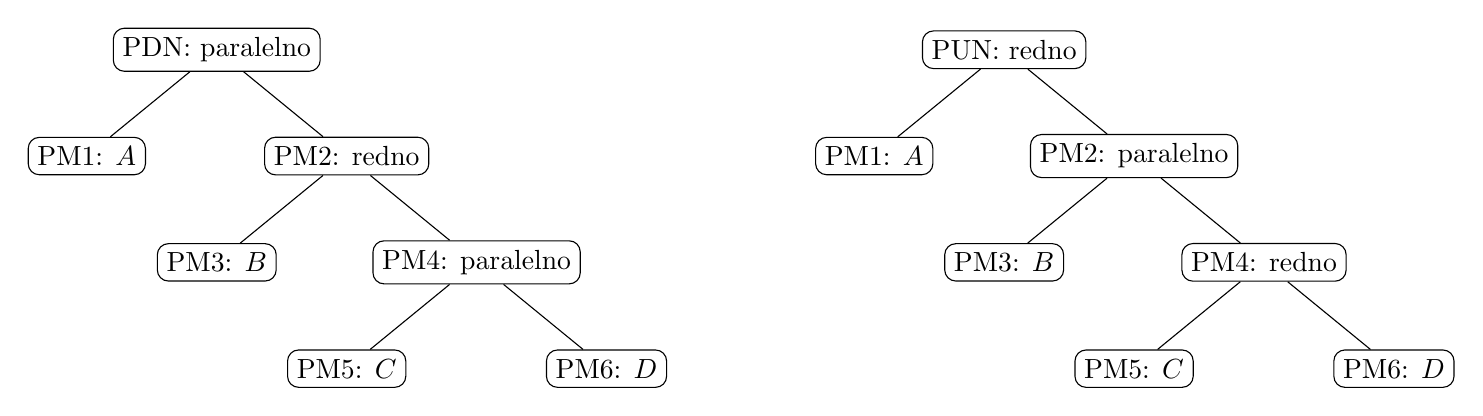
\begin{tikzpicture}[every node/.style={draw,rounded corners,align=center},level distance=1.35cm,sibling distance=3.3cm]
\node{PDN: paralelno}
 child{node{PM1: $A$}}
 child{node{PM2: redno}child{node{PM3: $B$}}child{node{PM4: paralelno}child{node{PM5: $C$}}child{node{PM6: $D$}}}};
\begin{scope}[xshift=10cm]
\node{PUN: redno}
 child{node{PM1: $A$}}
 child{node{PM2: paralelno}child{node{PM3: $B$}}child{node{PM4: redno}child{node{PM5: $C$}}child{node{PM6: $D$}}}};
\end{scope}\end{tikzpicture}
\end{document}
